\graphicspath{{content/2_design/figures/}}
\section{Battery Charger}

\subsection{Configuration}

The supplied battery charger circuit and PCB will be used, with the need to find the relevant resistor values.
The circuit has a diode-protected voltage regulator near the input to regulate the 12 V supply down. Then, a current-limiting
resistor is used to limit the charging current to the battery. Finally, a low-side NMOS control switch is used to control a high-side
PMOS current switch, which charges the battery through a diode.

\subsection{Voltage and Current Considerations}

The battery's voltage and current requirements need to be considered. For cycle use, the battery should be charged at between
7.30 and 7.40 volts, with a maximum current of 2.10 A. For this project, however, it is specified that the circuit should only charge
at 0.1C relative to a 4 Ah battery, and therefore a current limit of 400 mA should be adhered to. Lastly, once the cycle voltage has
been reached, a maximum of 0.001C current should be allowed into the battery to prevent overcharge, which equates to 4 mA.

\subsection{Design}

Resistor values in Figure \ref{fig:batteryCharger_circuitDiagram} should now be chosen, as well as transistor components.
The IRF9Z24 P-channel MOSFET will be used for M1 due to its continuous current capability of 8.5 A
and its low $R_{DS(on, max)}$ of $\SI{175}{\milli\ohm}$ causing a negligible ($\SI{4}{mV}$) voltage drop \cite{datasheetIRF9Z24N}.
The 1N5819 diode will be used for both D1 and D2 due to its low turn-on voltage and its high current capabilities.
The 2N7000 NMOS transistors will be used for M2, which has no specific requirements. Resistor values may now be calculated:

\begin{itemize}
    \item The output impedance seen by the battery is $R_o = R_1 \times (1 + \frac{R_4}{R_2})$ \cite{datasheet1N5819}.
          The regulator can be modeled as a voltage source $V_{reg}$ with resistance $R_o = \frac{V_{reg} - V_{diode} - V_{bat}}{I_{bat}}$.
          To cater for the maximum floating current, condition $R_o > \frac{V_{reg} - V_{diode} - V_{bat(full)}}{\SI{4}{mA}}$ must be met,
          and to cater for a high initial current up to $\SI{400}{mA}$, $R_o > \frac{V_{reg} - V_{diode} - V_{bat(empty)}}{\SI{400}{mA}}$.
    \item Choose $V_{bat(full)} = \SI{7.4}{V}$, $\therefore I_{bat} \leq \SI{4}{mA}$ and $V_{diode} \approx \SI{0.15}{V}$ \cite{datasheet1N5819}.
          Choose $V_{bat(empty)} = \SI{6.0}{V}$, $\therefore I_{bat} \leq \SI{400}{mA}$ and $V_{diode} \approx \SI{0.35}{V}$. Using the above,
          $\frac{V_{reg} - \SI{7.55}{V}}{\SI{4}{mA}} < R_o$ and $\frac{V_{reg} - \SI{6.35}{V}}{\SI{400}{mA}} < R_o$.
          Using graphing software, one solution is $R_o = \SI{3}{\ohm}$ with $V_{reg} \leq \SI{7.56}{V}$ yielding $I_{empty} \leq \SI{3.33}{mA}$ and $I_{full} \leq \SI{400}{mA}$.
    \item $R_1$, $R_2$ and $R_4$ can now be selected using $V_{reg} = V_{ref} (1 + \frac{R_4}{R_2}) \approx \SI{7.56}{V}$ and $R_o = R_1 (1 + \frac{R_4}{R_2}) > \SI{3}{\ohm}$.
          Now, $\frac{R_4}{R_2} = 5.05$ and $R_1 = \SI{0.496}{\ohm}$. Choose $R_1 = \SI{1}{\ohm} || \SI{1}{\ohm}$.
          Choose $R_4 = \SI{270}{\ohm}$ and $R_2 = \SI{1.5}{\kilo\ohm} || \SI{15}{\kilo\ohm}$ so that $V_{reg} = \SI{7.56}{V}$
\end{itemize}

\begin{figure}[!htb]
  \centering
  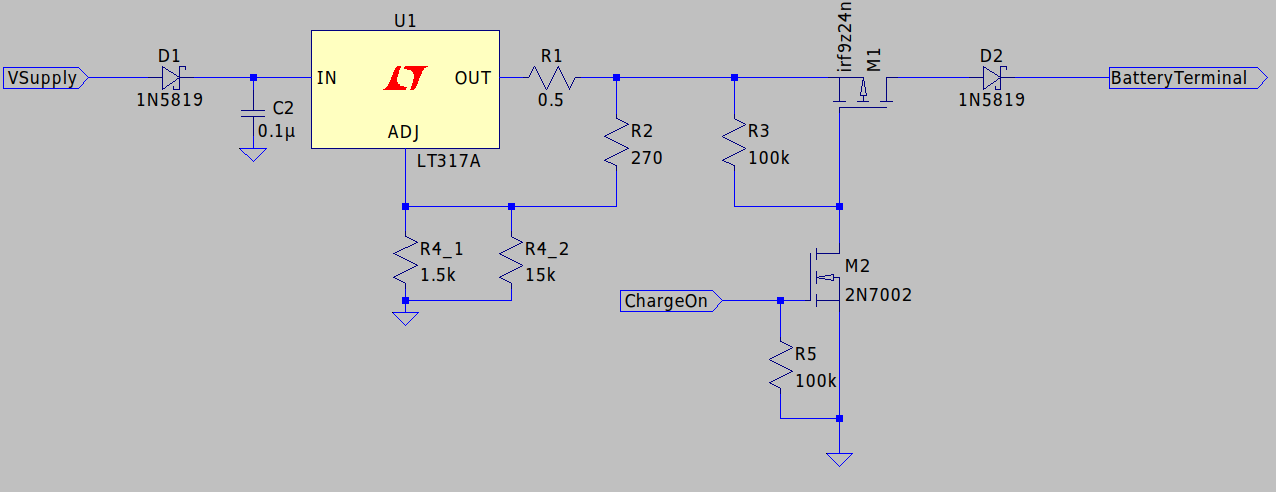
\includegraphics[width=0.6\textwidth]{batteryCharger_circuitDiagram}
  \caption{Battery Charger Circuit Diagram}
  \label{fig:batteryCharger_circuitDiagram}
\end{figure}